\begin{lstlisting}
p134 1 3 4 5 6 7
\end{lstlisting}
\begin{exercise}
\begin{figure}[H]
\centering
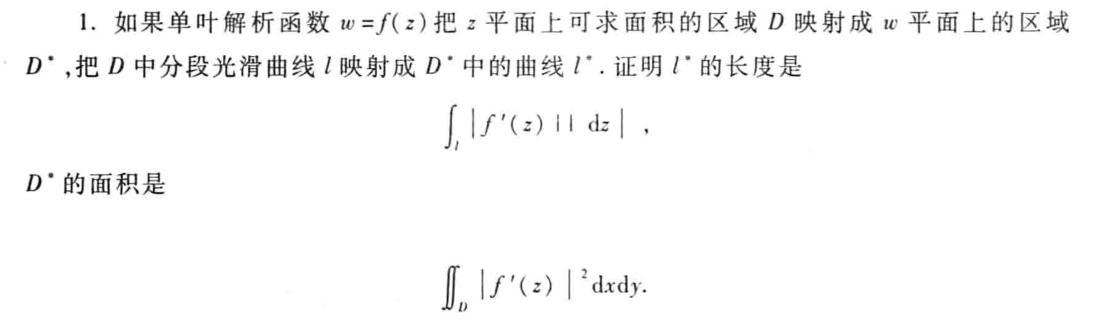
\includegraphics[width=\textwidth]{hw12-2025051912.png}
% \caption{}
\label{}
\end{figure}
\end{exercise}
Consider the parameterization of $l$,
\[
\gamma:[0,1]\to l\subset D
\]
Then the parameterization of $l^{*}$ is
\[
f\circ \gamma:[0,1]\to l\to l^{*}\subset D^{*}
\]
Since $w=f(z)$ is injective, the path $f\circ\gamma$ is well-defined simple closed curve. Then
\[
\begin{aligned}
\text{the length of }l^{*} & =\ell(f\circ \gamma) \\
 & =\int_{0}^{1} \lvert (f\circ \gamma)'(t) \rvert  \, \mathrm{d}t \\
 & =\int_{0}^{1} \lvert f'(\gamma(t)) \rvert \cdot \lvert \gamma'(t) \rvert  \, \mathrm{d}t 
\end{aligned} 
\]
On the other hand,
\[
\int_{l}^{} \lvert f'(z) \rvert  \, \lvert \mathrm{d}z \rvert  =\int_{\gamma}^{} \lvert f'(z) \rvert  \, \lvert \mathrm{d}z \rvert =\int_{0}^{1} \lvert f'(\gamma(t)) \rvert \cdot   \, \lvert \mathrm{d}\gamma(t) \rvert  =\int_{0}^{1} \lvert f'(\gamma(t)) \rvert \cdot \lvert \gamma'(t) \rvert  \, \mathrm{d}t 
\]
Therefore
\[
\text{the length of }l^{*}=\int_{l}^{} \lvert f'(z) \rvert  \, \lvert \mathrm{d}z \rvert  
\]
Denote $w=f(z)=u(x,y)+iv(x,y)$ ,where $z=x+iy$。

The area $A(D^*)$ of the region $D^*$ in the $w$-plane can be obtained by variable substitution using the Jacobian determinant:
\[
A(D^*) = \iint_{D^*} du\ dv
\]
According to the variable substitution formula for double integrals, we have:
\[
du\ dv = \left| \frac{\partial(u,v)}{\partial(x,y)} \right| dx\ dy
\]
where $\frac{\partial(u,v)}{\partial(x,y)}$ is the Jacobian determinant:
\[
\frac{\partial(u,v)}{\partial(x,y)} = \left| \begin{array}{cc} \frac{\partial u}{\partial x} & \frac{\partial u}{\partial y} \\ \frac{\partial v}{\partial x} & \frac{\partial v}{\partial y} \end{array} \right| = \frac{\partial u}{\partial x} \frac{\partial v}{\partial y} - \frac{\partial u}{\partial y} \frac{\partial v}{\partial x}
\]
Since $f(z)$ is an analytic function, its real part $u(x,y)$ and imaginary part $v(x,y)$ satisfy the Cauchy-Riemann equations:
\[
\frac{\partial u}{\partial x} = \frac{\partial v}{\partial y}
\]
\[
\frac{\partial u}{\partial y} = -\frac{\partial v}{\partial x}
\]
Substituting the Cauchy-Riemann equations into the Jacobian determinant:
\[
\frac{\partial(u,v)}{\partial(x,y)} = \left( \frac{\partial u}{\partial x} \right)^2 - \left( -\frac{\partial v}{\partial x} \right) \frac{\partial v}{\partial x} = \left( \frac{\partial u}{\partial x} \right)^2 + \left( \frac{\partial v}{\partial x} \right)^2
\]
We know that the complex derivative $f'(z)$ can be expressed as:
\[
f'(z) = \frac{\partial u}{\partial x} + i \frac{\partial v}{\partial x}
\]
Therefore, the square of the modulus of the complex derivative is:
\[
|f'(z)|^2 = \left( \frac{\partial u}{\partial x} \right)^2 + \left( \frac{\partial v}{\partial x} \right)^2
\]
So, the value of the Jacobian determinant is equal to $|f'(z)|^2$:
\[
\left| \frac{\partial(u,v)}{\partial(x,y)} \right| = |f'(z)|^2
\]
Now we substitute this result back into the area integral formula:
\[
A(D^*)=\iint_D\left|\frac{\partial(u,v)}{\partial(x,y)}\right|dxdy=\iint_D|f'(z)|^2dxdy
\]
This proves the second conclusion.

\begin{exercise}
\begin{figure}[H]
\centering
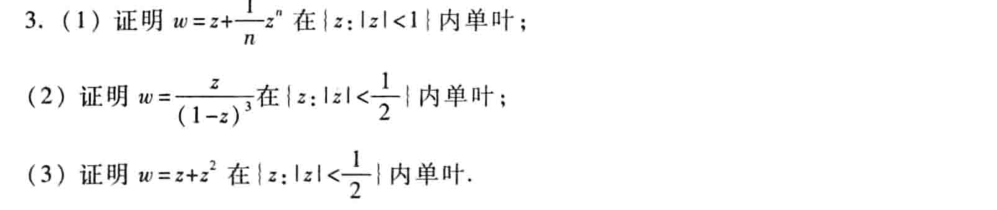
\includegraphics[width=\textwidth]{1-hw12-2025051912.png}
% \caption{}
\label{}
\end{figure}
\end{exercise}
(1)
For $z_1, z_2\in \{ z:\lvert z \rvert<1 \}$, if
\[
z_1+\frac{1}{n}z_1^{n}=z_2+\frac{1}{n}z_2^{n}
\]
Then
\[
z_1-z_2=\frac{1}{n}(z_2^{n}-z_1^{n})
\]
\[
\begin{aligned}
\lvert z_1-z_2 \rvert &  =\frac{1}{n}\lvert z_2^{n}-z_1^{n} \rvert =\frac{1}{n}\lvert (z_2-z_1)(z_2^{n-1}+z_2^{n-2}z_1+\dots+z_1^{n-1}) \rvert  \\
 & \leq \frac{1}{n}\lvert z_2-z_1 \rvert (\lvert z_2 \rvert ^{n-1}+\lvert z_2 \rvert ^{n-2}\lvert z_1 \rvert +\dots+\lvert z_1 \rvert ^{n-1}) \\
 & <\frac{1}{n}\lvert z_2-z_1 \rvert \cdot n  \\
 & =\lvert z_2-z_1 \rvert  
\end{aligned}
\]
Thus $z_1=z_2$. $w$ is injective.

(2)
For $z_1, z_2\in \left\{  z:\lvert z \rvert<\frac{1}{2}  \right\}$, if
\[
\frac{z_1}{(1-z)^{3}}=\frac{z_2}{(1-z_2)^3}
\]
Then
\[
z_1-3z_1z_2+3z_1z_2^2-z_1z_2^3=z_2-3z_2z_1+3z_2z_1^2-z_2z_1^3
\]
\[
\begin{aligned}
\lvert z_1-z_2 \rvert  & =\lvert 3z_1z_2(z_1-z_2)+z_1z_2(z_2-z_1)(z_1+z_2) \rvert  \\
 & \leq 3\lvert z_1z_2 \rvert \lvert z_1-z_2 \rvert +\lvert z_1z_2 \rvert \lvert z_1+z_2 \rvert \lvert z_2-z_1 \rvert  \\
 & < \frac{3}{4}\lvert z_1-z_2 \rvert +\frac{1}{4}\lvert z_1-z_2 \rvert =\lvert z_1-z_2 \rvert 
\end{aligned}
\]
Thus $z_1=z_2$. $w$ is injective.

(3)
For $z_1, z_2\in \left\{  z:\lvert z \rvert<\frac{1}{2}  \right\}$, if
\[
z_1+z_1^2=z_2+z_2^2
\]
Then
\[
\lvert z_1-z_2 \rvert =\lvert z_1^2-z_2^2 \rvert =\lvert z_1-z_2 \rvert \lvert z_1+z_2 \rvert \leq (\lvert z_1 \rvert +\lvert z_2 \rvert )\lvert z_1-z_2 \rvert <\lvert z_1-z_2 \rvert 
\]
Thus $z_1=z_2$. $w$ is injective.

\begin{exercise}
\begin{figure}[H]
\centering
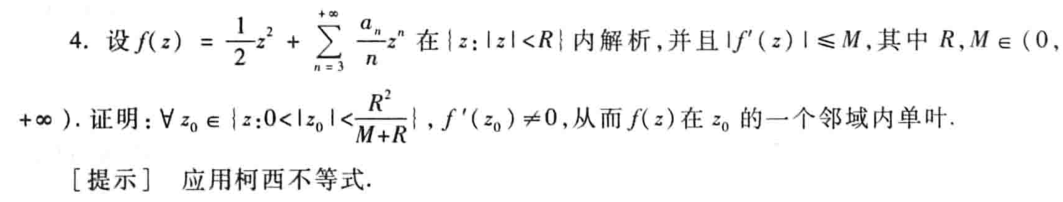
\includegraphics[width=\textwidth]{3-hw12-2025051912.png}
% \caption{}
\label{}
\end{figure}
\end{exercise}
Denote
\[
g(z)\coloneqq f'(z)=z+\sum_{n=2}^{\infty} a_{n+1}z^{n}
\]
Then
\[
\lvert g(z) \rvert \leq M,\forall \lvert z \rvert <R
\]
By Cauchy's formula,
\[
a_{n+1}=\frac{1}{2\pi i}\oint_{\lvert z \rvert =r}\frac{g(\xi)}{\xi^{n+1}}d\xi
\]
where $r\in(0,R)$. Then
\[
\lvert a_{n+1} \rvert \leq \frac{1}{2\pi }\oint_{\lvert z \rvert =r}\left\lvert  \frac{g(\xi)}{\xi^{n+1}}  \right\rvert d\xi\leq \frac{1}{2\pi}\cdot2\pi r \cdot\frac{M}{r^{n+1}}=\frac{M}{r ^{n}}
\]
Let $r\to R$, then
\[
\lvert a_{n+1} \rvert \leq \frac{M}{R^{n}}
\]
Thus for any $z\in \left\{  z:\lvert z \rvert<\frac{R^2}{M+R}  \right\}$,
\[
\begin{aligned}
\left\lvert  \sum_{n=2}^{\infty} a_{n+1}z^{n} \right\rvert & \leq \sum_{n=2}^{\infty} \underbrace{ \lvert a_{n+1} \rvert }_{ \leq \frac{M}{R^{n}} } \lvert z \rvert ^{n}  \\
 & \leq \sum_{n=2}^{\infty} M\left\lvert  \frac{z}{R}  \right\rvert ^{n} \\
 & =\lvert z \rvert \cdot\frac{M}{R}\sum_{n=2}^{\infty} \left\lvert  \frac{z}{R}  \right\rvert ^{n-1} \\
 & <\lvert z \rvert \cdot\frac{M}{R}\sum_{n=2}^{\infty} \left\lvert  \frac{R}{M+R}  \right\rvert ^{n-1}  \\
 & =\lvert z \rvert \cdot \frac{M}{R}\cdot\frac{\frac{R}{M+R}}{1-\frac{R}{M+R}} \\
 & =\lvert z \rvert 
\end{aligned}
\]
By Rouche's theorem, $z$ and $g(z)$ has the same numbers of zero's in $\left\{  z:\lvert z \rvert<\frac{R^2}{M+R}  \right\}$, i.e. only $1$ zero. As $g(0)=0$, $g(z)$ has no zero in $\left\{  z:0<\lvert z \rvert<\frac{R^2}{M+R}  \right\}$.

Assume that $f$ is not injective in $\left\{  z:0<\lvert z \rvert<\frac{R^2}{M+R}  \right\}$. There exists $z_1,z_2$ s.t.
\[
f(z_1)=f(z_2)
\]
By the MVT, there exists $\theta\in[0,1]$, s.t.
\[
f'(\theta z_1+(1-\theta)z_2)=0
\]
By the convexity of $\left\{  z:0<\lvert z \rvert<\frac{R^2}{M+R}  \right\}$,
\[
\theta z_1+(1-\theta)z_2\in \left\{  z:0<\lvert z \rvert <\frac{R^2}{M+R}   \right\}
\]
is a zero of $g(z)$, whihc is a contradiction. Hence, $f$ is injective in $\left\{  z:0<\lvert z \rvert<\frac{R^2}{M+R}  \right\}$; for any $z_0\in \left\{  z:0<\lvert z \rvert<\frac{R^2}{M+R}  \right\}$, it is an interior point of $\left\{  z:0<\lvert z \rvert<\frac{R^2}{M+R}  \right\}$, thus has a neighborhood where $f$ is injective.

\begin{exercise}
\begin{figure}[H]
\centering
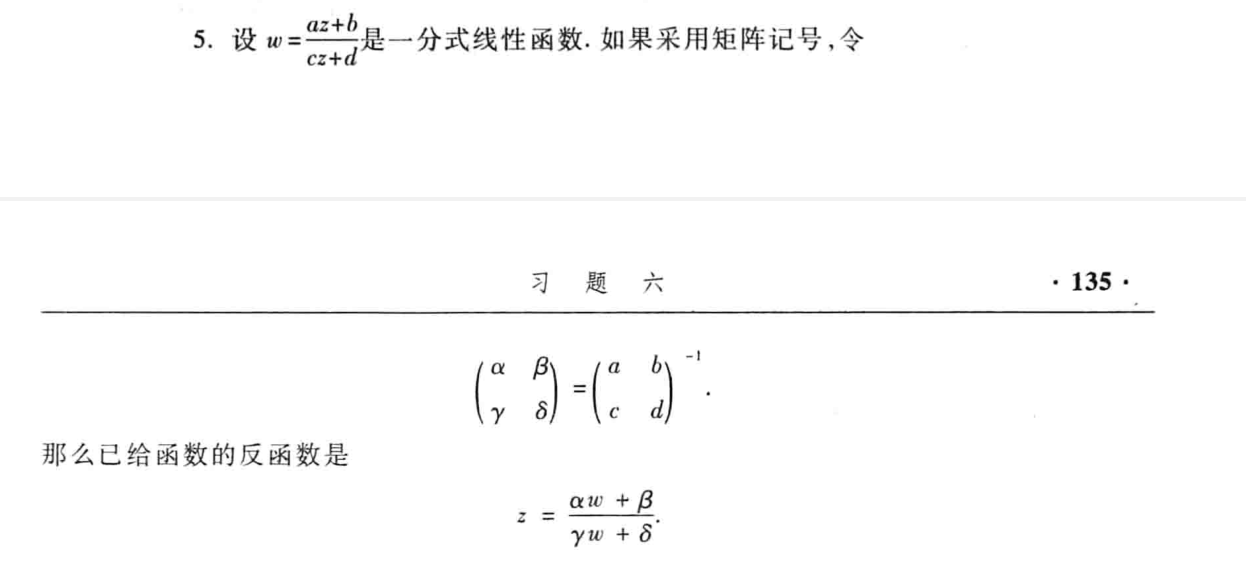
\includegraphics[width=\textwidth]{hw12-2025051920.png}
% \caption{}
\label{}
\end{figure}
\end{exercise}
\[
\begin{pmatrix}
\alpha & \beta \\
\gamma & \delta 
\end{pmatrix}=\left(
\begin{array}{cc}
 \frac{d}{a d-b c} & -\frac{b}{a d-b c} \\
 -\frac{c}{a d-b c} & \frac{a}{a d-b c} \\
\end{array}
\right)
\]
Then
\[
\begin{aligned}
\frac{a\frac{\alpha w+\beta}{\gamma w+\delta}+b}{c\frac{\alpha w+\beta}{\gamma w+\delta}+d} & =\frac{a\alpha w+a\beta+b\gamma w+b\delta}{c\alpha w+c\beta+d\gamma w+d\delta} \\
 & =\frac{a\frac{d}{a d-b c} w+a\left( -\frac{b}{a d-b c} \right)+b\left(  -\frac{c}{a d-b c} \right) w+b\frac{a}{a d-b c}}{c\frac{d}{a d-b c} w+c\left( -\frac{b}{a d-b c} \right)+d\left(  -\frac{c}{a d-b c} \right) w+d\frac{a}{a d-b c}} \\
 & =\frac{adw-ab-bcw+ab}{cdw-bc-cdw+ad} \\
 & =w
\end{aligned}
\]
\[
\begin{aligned}
\frac{\alpha\frac{az+b}{cz+d}+\beta}{\gamma\frac{az+b}{cz+d}+\delta} & =\frac{\frac{d}{a d-b c}\frac{az+b}{cz+d}-\frac{b}{a d-b c}}{-\frac{c}{a d-b c}\frac{az+b}{cz+d}+\frac{a}{a d-b c}} \\
 & =\frac{adz+bd-bcz-bd}{-acz-bc+acz+ad} \\
 & =z 
\end{aligned}
\]
Thus the inverse of $w=\frac{az+b}{cz+d}$ is
\[
z=\frac{\alpha w+\beta}{\gamma w+\delta}
\]
\begin{exercise}
\begin{figure}[H]
\centering
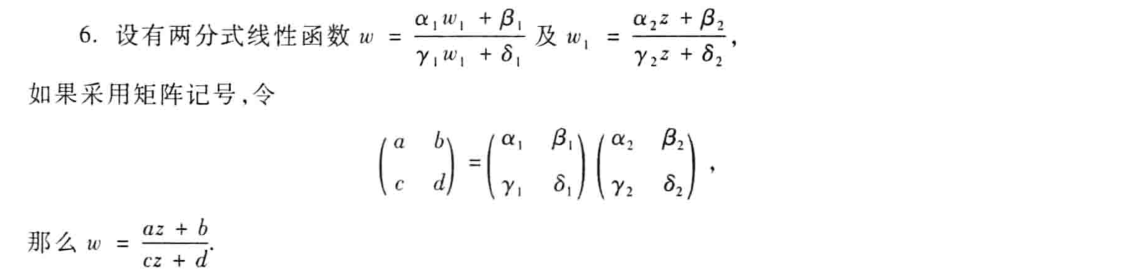
\includegraphics[width=\textwidth]{5-hw12-2025051912.png}
% \caption{}
\label{}
\end{figure}
\end{exercise}
\[
\begin{pmatrix}
a & b \\
c & d
\end{pmatrix} = \begin{pmatrix}
\alpha_1 & \beta_1 \\
\gamma_1 & \delta_1
\end{pmatrix} \begin{pmatrix}
\alpha_2 & \beta_2 \\
\gamma_2 & \delta_2
\end{pmatrix}=\left(
\begin{array}{cc}
 \alpha _1 \alpha _2+\beta _1 \gamma _2 & \alpha _1 \beta _2+\beta _1 \delta _2 \\
 \alpha _2 \gamma _1+\gamma _2 \delta _1 & \beta _2 \gamma _1+\delta _1 \delta _2 \\
\end{array}
\right)
\]
\[
w=\frac{\alpha_{1}w_{1}+\beta_{1}}{\gamma_{1}w_{1}+\delta_{1}}\qquad w_{1}=\frac{\alpha_{2}z+\beta_{2}}{\gamma_{2}z+\delta_{2}}
\]
Then
\[
w=\frac{\alpha_{1}\frac{\alpha_{2}z+\beta_{2}}{\gamma_{2}z+\delta_{2}}+\beta_{1}}{\gamma_{1}\frac{\alpha_{2}z+\beta_{2}}{\gamma_{2}z+\delta_{2}}+\delta_{1}}=\frac{\alpha _1 \beta _2+\beta _1 \delta _2+\alpha _1 \alpha _2 z+\beta _1 \gamma _2 z}{\beta _2 \gamma _1+\delta _1 \delta _2+\alpha _2 \gamma _1 z+\gamma _2 \delta _1 z}=\frac{az+b}{cz+d}
\]
\begin{exercise}
\begin{figure}[H]
\centering
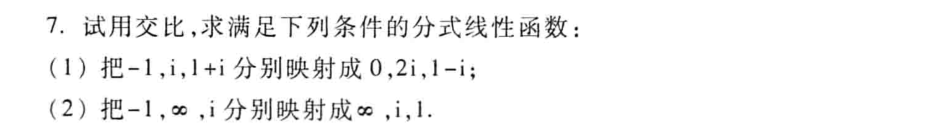
\includegraphics[width=\textwidth]{6-hw12-2025051912.png}
% \caption{}
\label{}
\end{figure}
\end{exercise}
\begin{figure}[H]
\centering
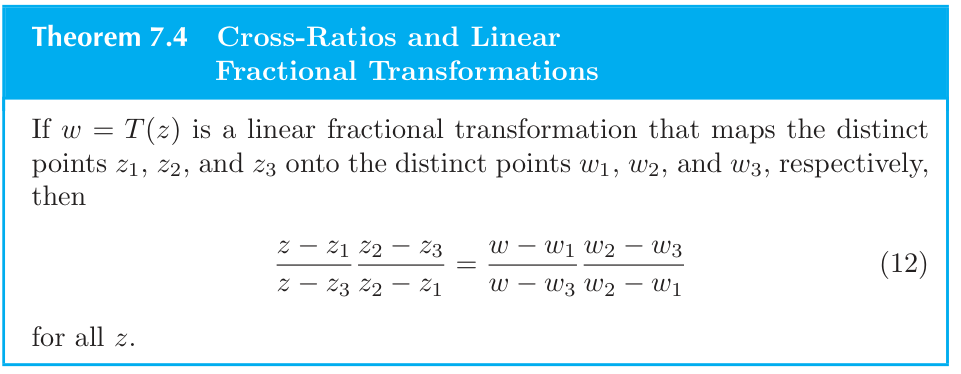
\includegraphics[width=\textwidth]{hw12-2025051921.png}
% \caption{}
\label{}
\end{figure}

(1)
\[
\frac{z-(-1)}{z-(1+i)}\cdot\frac{i-(1+i)}{i-(-1)}=\frac{w-0}{w-(1-i)}\cdot\frac{2i-(1-i)}{2i-0}
\]
Then
\[
w=\frac{(1-i) z+(1-i)}{(2+2 i) z+(2-3 i)}
\]
(2)
\[
\frac{z-(-1)}{z-i}\cdot\frac{\infty-i}{\infty-(-1)}=\frac{w-\infty}{w-1}\cdot\frac{i-1}{i-\infty}
\]
i.e.
\[
\frac{z+1}{z-i}=\frac{i-1}{w-1}
\]
Then
\[
w=\frac{i z+(2+i)}{z+1}
\]